% M11 partitioning & mesh-ordering report.
% Build:  module load texlive/live2025-gcc-13.3.0 && pdflatex m11_partitioning_report.tex (x2)
\documentclass[11pt,a4paper]{article}

\usepackage[utf8]{inputenc}
\usepackage[T1]{fontenc}
\usepackage{lmodern}
\usepackage[margin=22mm,top=18mm,bottom=18mm]{geometry}
\usepackage{amsmath,amssymb}
\usepackage{booktabs}
\usepackage{graphicx}
\usepackage{microtype}
\usepackage{parskip}
\usepackage{multirow}
\usepackage{titlesec}
\usepackage[hidelinks]{hyperref}

\titleformat{\section}{\normalfont\large\bfseries}{\thesection.}{0.6em}{}
\titlespacing*{\section}{0pt}{13pt}{5pt}
\titleformat{\subsection}{\normalfont\bfseries}{\thesubsection.}{0.5em}{}
\titlespacing*{\subsection}{0pt}{9pt}{3pt}
\setlength{\tabcolsep}{5pt}

\newcommand{\minconn}{\texttt{MINCONN}}
\newcommand{\contig}{\texttt{CONTIG}}

\title{\vspace{-12mm}\large\bfseries Mesh partitioning and node ordering for FESOM2/Kokkos:\\
measurements on CPU and GPU, and a procedure for adopting a new partition}
\author{\normalsize Technical report}
\date{\normalsize 13 August 2026 --- Levante (128-core CPU nodes, 4$\times$A100 GPU nodes; GH200 testbed)}

\begin{document}
\maketitle
\vspace{-6mm}

\subsection*{TL;DR}
\begin{itemize}\itemsep1pt
\item \textbf{GPU: a better mesh partition makes the model step 8--14\,\% faster} on three of
the four meshes tested (3.6\,\% on the fourth), and up to $19.7\,\%$ on DARS if a larger
change of the solution is accepted (Section~6). One factor dominates: the largest number of
neighbour subdomains any process exchanges halo data with. METIS can minimise it (option
\minconn), but FESOM calls METIS through \texttt{PartGraphRecursive}, which ignores that
option; calling \texttt{PartGraphKway} instead is a few-line change.
\item \textbf{CPU: 4--8\,\% faster}, from two different factors: allowing METIS a few percent
of imbalance in subdomain size (\texttt{UFACTOR=30} instead of the current 1), and using
newer partitioning programs (KaMinPar, Mt-KaHyPar) in place of METIS. The best CPU and GPU
partitions of the same mesh differ.
\item Partitions built with identical settings but different random seeds already give
slightly different solutions. We use the size of that scatter as the yardstick for every
recommended partition: most stay inside it; the exceptions are quantified in Section~6.
\item \textbf{Some new partitions crash the model} after hundreds of steps --- eight cases
here, one of them built with FESOM's current settings, and no property of the partition
predicts them. A new partition must complete 3{,}000 steps at its target process count before
use; if it fails, regenerate it with a different seed.
\item Renumbering the mesh nodes along a Hilbert curve pays only on CORE2 ($-5.8\,\%$
together with repartitioning); the other meshes are already well ordered.
\end{itemize}
\vspace{2pt}

\section{Summary}

A FESOM2 run reads which mesh nodes belong to which process from the \texttt{dist\_N} files
that ship with the mesh. Replacing those files changes nothing else --- no recompilation, no
namelist change, no effect on any other configuration --- so a better partition is the
cheapest speed-up available to an existing setup. It is also one that has never been tuned:
the partitioner has called METIS with the same options since its METIS-5 interface was written
in 2015, and one of the four meshes here ships partitions that our build still reproduces byte
for byte.

We generated several hundred partitions of four meshes --- with METIS under settings FESOM
does not currently use, with three other partitioning programs, and after two renumberings of
the mesh nodes --- and timed them against the shipped partitions on both backends of the
C++/Kokkos port.

The shipped partitions cost the GPU backend up to 20\,\% of the model step. Most of that is
recovered by a single METIS option, \minconn, which minimises the largest number of
neighbouring subdomains any process has and which no FESOM partition has ever had active,
because \texttt{METIS\_PartGraphRecursive} accepts the option and ignores it. The CPU backend
gains 4--8\,\%, from imbalance tolerance and from newer partitioning programs rather than from
\minconn; the two backends are best served by different partitions of the same mesh.

A partition change also perturbs the solution, and two properties of that perturbation
matter. It is usually no larger than the difference between two partitions built with the same
settings and different random seeds (Section~6). But in a minority of cases it is fatal: eight
of the partitions generated here make the model diverge after tens to hundreds of steps, one
of them built with FESOM's current settings, and no property computable from a partition
identifies them in advance (Section~5). Every new partition therefore has to be run before it
is trusted.

Meshes: CORE2 (127k surface nodes, 1$^\circ$), fArc (638k), DARS (3.16M), NG5 (7.40M, $\approx$5\,km).
All experiments are cold starts under JRA55 (1958) forcing from PHC climatology, at the largest
time step at which a cold start of the given mesh is stable: 1800\,s on CORE2, 900\,s on fArc,
120\,s on DARS, 180\,s on NG5.

\section{Candidates}

\textbf{METIS settings.} Switching the METIS call from \texttt{PartGraphRecursive} to
\texttt{PartGraphKway} makes three previously ignored options effective: the
communication-volume objective, contiguity of the subdomains (\contig), and \minconn, which
minimises the largest number of neighbouring subdomains any subdomain has. We swept these
together with \texttt{UFACTOR}, which sets how much the subdomains may differ in size (values
10, 30 and 100, i.e. 1, 3 and 10\,\%, against the 0.1\,\% FESOM uses now); with the node
weight $w = a + \mathrm{nlev}$ for $a$ between 0 and 100, which trades balancing the number of
surface nodes per process against balancing the number of wet layers; with two-level
hierarchical partitions; and with the METIS random seed. The Recursive call is not an
oversight: \texttt{fort\_part.c} documents that it produced the better partition on a test
mesh, and lists which options it ignores. That comparison predates the GPU backend.

\textbf{Other partitioning programs.} KaHIP, KaMinPar and Mt-KaHyPar, each given the same
weighted graph and the same sweep over $a$. FESOM does not interface to them; we exported the
graph METIS is given, partitioned it externally, and read the result back, so the comparison
is between partitions of one and the same graph.

\textbf{Node renumbering.} Renumbering the mesh nodes along a Hilbert space-filling curve, and
alternatively by reverse Cuthill--McKee, so that nodes close in the mesh are close in memory.
Unlike a partition, a renumbering changes the mesh files themselves, so every reference
solution pinned to the old numbering must be re-established.

\textbf{A second architecture.} The best GPU settings were re-timed on DKRZ's GH200 nodes
(dolpung), whose interconnect cannot register GPU memory; halos there are staged through pinned
host buffers, which prices communication differently than the A100 fabric does.

\section{Measurement procedure}

Timing runs place all candidates in a single job allocation and interleave repetitions, so that
node-to-node and time-of-day variation affects every candidate alike. Each run integrates 300
steps; we quote the best of $N$ repetitions, as a percentage of the shipped partition's time per
step. The mesh-definition files are verified byte-identical across candidates before the job
starts, so the candidates differ in the decomposition only.

A timing result is accepted only after two further tests.

\emph{Stability.} The candidate must complete 3{,}000 steps at the process count at which it
will be used. Because the time step is set by the mesh, that is two months of model time on
CORE2, one on fArc, but only four to six days on DARS and NG5 --- a bound on the test, not a
claim about long integrations. It exists because it fails in practice: a DARS partition that
had won its timing comparison by 4.5\,\% diverged between step 150 and step 3{,}000 while the
shipped partition ran cleanly.

\emph{Size of the solution change.} A different partition sums the same terms in a different
order, and the resulting round-off differences grow at fronts, so a new partition cannot be
asked to reproduce the reference solution bit for bit. The question is how large its
difference from the reference is compared with the difference any other partition would
produce. We therefore rebuild the shipped partition with three or more different METIS random
seeds --- checking in each case that the result really is a different partition --- run twenty
steps with each, and compare the candidate's rms difference from the reference in temperature,
salinity and sea-surface height with the range those seed partitions span. Section~6 reports
each candidate on that scale. Quantiles and maxima of the difference fields are recorded as
well.

Twenty steps from a cold start measure whether a partition change is detectable at all; they
say nothing about a multi-decade integration. Section~6 returns to this.

Partitions we recommend are packaged by a tool that refuses any \texttt{dist\_N} without a
recorded clean 3{,}000-step run at exactly $N$ processes.

\section{Speed}

Figure~\ref{fig:board} and Table~\ref{tab:board} give the best candidate at each mesh and
process count, with the setting that produced it. Every gain re-measured over 3{,}000 steps
came back equal to or larger than its 300-step value (Fig.~\ref{fig:mech}b; $-18.6$ to
$-19.7\,\%$ on DARS GPU is the largest change), so the short timing runs do not overstate the
effect.

\begin{figure}[t]\centering
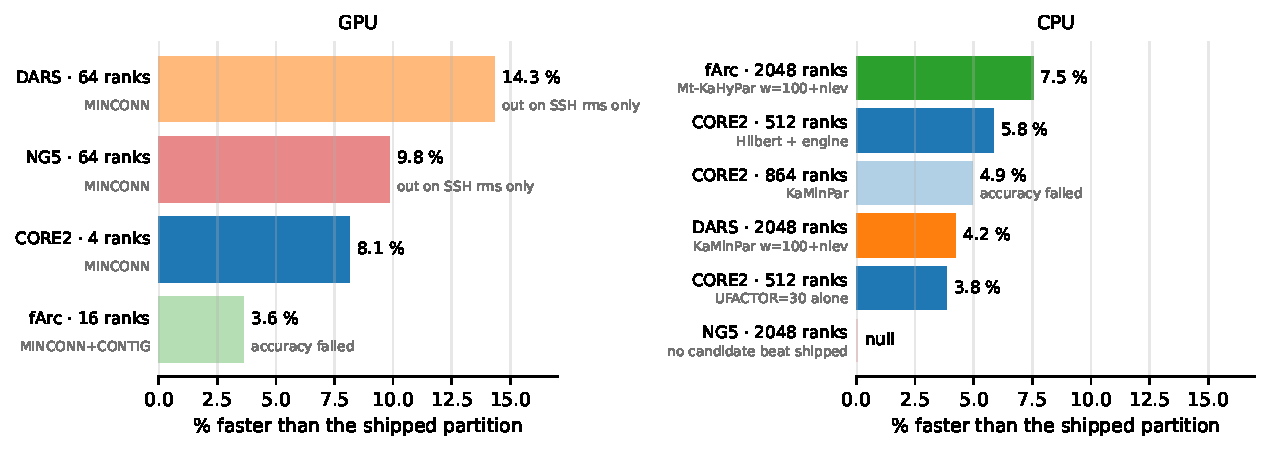
\includegraphics[width=\textwidth]{fig_m11_board.pdf}
\caption{\small Best candidate partitions per mesh and process count, as a percentage faster
than the shipped partition. Gray text under each label is the setting that produced the
candidate. All candidates shown completed the 3{,}000-step run. The fill codes the size of
their solution change against the seed-partition scatter of Section~6: solid = within it,
single-hatched = larger in sea-surface height only, cross-hatched = larger in temperature or
salinity. Mesh colors recur in Figs.~\ref{fig:mech}, \ref{fig:gh200} and \ref{fig:dist}.}
\label{fig:board}
\end{figure}

\begin{table}[h]\centering\footnotesize
\setlength{\tabcolsep}{3.4pt}
\begin{tabular}{llrlll}
\toprule
mesh & processes & gain & setting & 3{,}000 steps & solution change vs seed scatter \\
\midrule
DARS  & 64 GPU   & $\mathbf{-19.7\,\%}$ & \minconn+\contig+\texttt{UF=30} & clean & T rms $+13\,\%$, T max 16.2 vs 6.4--8.8 \\
DARS  & 64 GPU   & $\mathbf{-14.3\,\%}$ & \minconn            & clean & ssh rms $+11\,\%$; T, S within \\
NG5   & 64 GPU   & $\mathbf{-9.8\,\%}$  & \minconn             & clean & ssh rms $+8\,\%$; T, S within \\
CORE2 & 4 GPU     & $\mathbf{-8.1\,\%}$  & \minconn             & clean & below every seed partition \\
fArc  & 16 GPU   & $-3.6\,\%$           & \minconn+\contig     & clean & T rms $+33\,\%$, ssh $+68\,\%$ \\
\midrule
fArc  & 2048 CPU & $\mathbf{-7.5\,\%}$  & Mt-KaHyPar $w{=}100{+}\mathrm{nlev}$ & clean & within (4 seeds) \\
CORE2 & 512 CPU  & $\mathbf{-5.8\,\%}$  & Hilbert renumbering + KaHIP & clean & within \\
DARS  & 2048 CPU & $\mathbf{-4.2\,\%}$  & KaMinPar $w{=}100{+}\mathrm{nlev}$ & clean & below every seed partition (T, S) \\
CORE2 & 864 CPU  & $-4.9\,\%$           & KaMinPar             & clean & salinity rms $+24\,\%$ \\
CORE2 & 512 CPU  & $-3.8\,\%$           & \texttt{UFACTOR=30} & clean & within \\
NG5   & 2048 CPU & none                 & ---                  & --- & --- \\
\bottomrule
\end{tabular}
\caption{\small Best candidates per mesh and process count, relative to the shipped partition,
at the time step given in Section~1. The last column gives the twenty-step rms difference from
the reference where it exceeds what different METIS seeds produce, with the field responsible;
Section~6 gives the numbers and what is known about their cause. On NG5 at 2{,}048 CPU
processes no candidate was faster than the shipped partition.}
\label{tab:board}
\end{table}

\subsection{What the two backends pay for}

Across the nine groups of timed candidates, the number of neighbour subdomains a process
exchanges with is the only quantity computable from the partition that correlates positively
with GPU step time. Every quantity measuring how much data is sent --- edge cut, halo size,
replicated elements --- correlates negatively: on the GPU, candidates that send more data are
faster if they send it to fewer neighbours. That is the behaviour of a machine paying per
message rather than per byte, and \minconn\ is the METIS objective that reduces the number of
messages.

Across meshes the GPU gain follows the reduction in the \emph{largest} neighbour count, not
the mean (Fig.~\ref{fig:mech}a): the mean falls by a similar fraction at all three points and
so cannot order them, while the maximum ranges from $-14\,\%$ (fArc, $-3.6\,\%$ gain) to
$-42\,\%$ (DARS, $-18.6\,\%$). The maximum is the relevant statistic because each step waits
for the slowest process. Section~4.3 shows that the coefficient of this relation is a property
of the interconnect, not a constant.

\begin{figure}[t]\centering
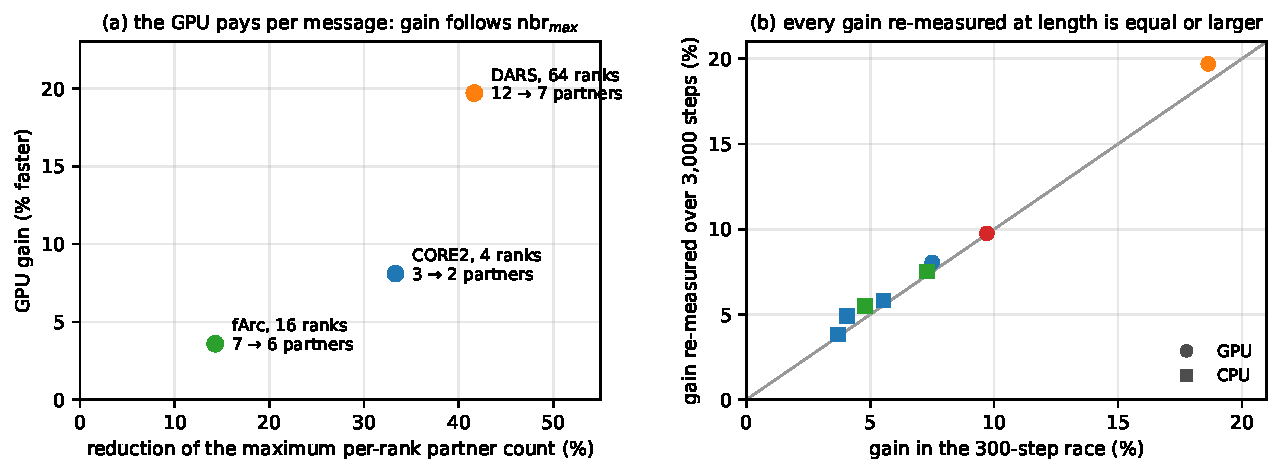
\includegraphics[width=\textwidth]{fig_m11_mechanism.pdf}
\caption{\small (a) GPU gain against the fractional reduction of the largest number of
neighbour subdomains any process has, annotated with the counts before and after. (b) Gain
measured over 300 steps against the same candidate's gain re-measured over 3{,}000 steps, for
the eight candidates measured both ways; the line marks equality, circles are GPU points,
squares CPU, and colors identify the mesh as in Fig.~\ref{fig:board}.}
\label{fig:mech}
\end{figure}

On the CPU no quantity computable from the partition orders the candidates: for imbalance,
edge cut and neighbour count alike, the rank correlation with step time straddles zero across
the timed groups, so CPU candidates have to be timed. Two regularities survive. An external
program won at every CPU point with 512 or more processes. And the same two options that gain
five percentage points on DARS GPU when added to \minconn\ --- \contig\ and \texttt{UFACTOR=30}
--- lose one to two on DARS CPU.

\subsection{Node renumbering pays only on CORE2}

On CORE2, Hilbert renumbering is worth $-1.2$ to $-2.4\,\%$ on CPU and $-5.0\,\%$ on a single
GPU node, and combines almost additively with repartitioning ($-5.8\,\%$ at 512 processes).
The other meshes gain nothing: 88\,\% of the nodes an element gathers from are already
adjacent in memory, against 27.6\,\% on CORE2. Since renumbering forces every reference
solution to be re-established (Section~2), it is worth taking only where that cost is
acceptable; repartitioning carries no such cost.

\subsection{The second architecture}

On a single GH200 node the CORE2 gain reproduces at $-8.9\,\%$ against $-8.1\,\%$ on A100
(two independent jobs, agreeing within 0.6 percentage points), so it is not specific to A100
hardware. It does not survive the move to several nodes (Fig.~\ref{fig:gh200}). We registered
a prediction before the job ran that DARS on 64 GH200 processes would exceed its A100 gain of
$-18.6\,\%$; the measured effect is $-1$ to $-3\,\%$, and fArc on four nodes shows no effect
at five repetitions. On this machine the per-message cost \minconn\ removes therefore sits in
the intra-node path, where halos are staged through host buffers, and not in the inter-node
fabric. Multi-node gains have to be measured on each interconnect.

These jobs also showed that quoting the best of $N$ repetitions is biased when the reference
partition is the noisiest configuration, as it was there: best-of-4 made every fArc candidate
look 0.8--2.3\,\% slower than the reference while the medians put them within 0.6\,\%. Where
the scatter differs between configurations we report medians as well.

\begin{figure}[t]\centering
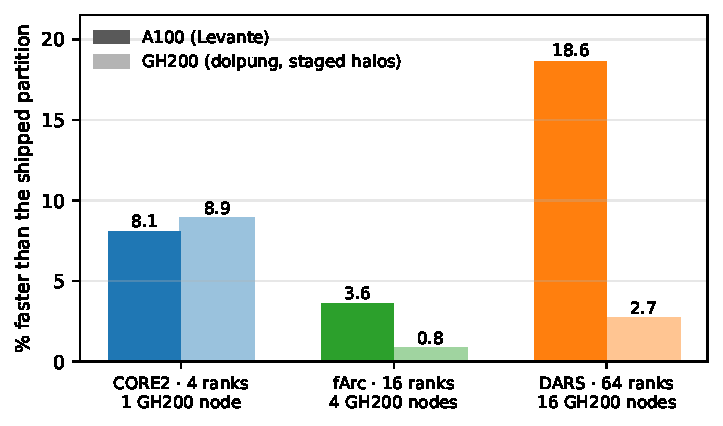
\includegraphics[width=0.62\textwidth]{fig_m11_gh200.pdf}
\caption{\small The three GPU settings re-timed on GH200 (hatched) against their A100 values
(solid), with the GH200 node count under each pair. The GH200 values for fArc and DARS are
medians, because the shipped partition was the noisiest configuration in those jobs and the
best-of-$N$ estimator is then biased; the fArc value is indistinguishable from zero at the
measured noise level.}
\label{fig:gh200}
\end{figure}

\section{Some repartitioned meshes crash the model}

Eight of the partitions generated here make the model diverge: on NG5, \minconn\ candidates at
2{,}048 and at 64 processes and a \texttt{UFACTOR=30} candidate at 64; on DARS, \minconn\
candidates at 2{,}048; and, also on DARS at 2{,}048, one partition built with FESOM's current
settings and nothing changed but the METIS random seed, which diverged within fourteen steps.
The failure is local in every case: salinity runs away at one location --- 41 to 57 over four
steps in the seed case --- while the global diagnostics stay normal and the mean sea level even
decreases.

Three properties of these failures matter in practice.

They have no signature in the partition. In the NG5 group, the partitions that later diverged
scored better than the survivors on every quantity we computed, including imbalance, edge cut,
the number of disconnected pieces and the number of isolated nodes.

Short tests do not find them. A five-step run passes on a partition that diverges at step 71,
and the 150-step timing runs passed on a partition that diverged before step 3{,}000. The
3{,}000-step run of Section~3 caught every failure listed above; nothing shorter would have.

The failure belongs to the individual partition, not to the settings. On both meshes where a
winning candidate diverged, rebuilding it with the same settings and a different METIS seed
gave a partition that ran --- the full 3{,}000 steps on DARS, the 150-step timing run on NG5
--- in one case with a worse edge cut than the partition that had failed. Conversely, the
settings of the fastest DARS GPU candidate give a sound partition at 64 processes and a fatally unstable
one at 2{,}048.

Because FESOM's current settings produced one of the eight, the partitions now in production
are not safer by construction; they have simply been run. The 3{,}000-step test is therefore
the price of adopting \emph{any} new partition, not a surcharge on the options recommended
here.

\section{How much the solution changes}

A new partition changes the solution. The question is how much, relative to what a user
already accepts without knowing it: rebuilding the same partition with a different METIS seed
changes the solution too. Figure~\ref{fig:dist} places every candidate on that scale, field by
field. The scale is not transferable between meshes --- the seed partitions themselves span a
factor 1.05 in salinity rms on DARS at 2{,}048 processes and a factor 3.9 on CORE2 at 864 ---
so a fixed rms threshold would be meaningless. Four cases occur.

\begin{figure}[t]\centering
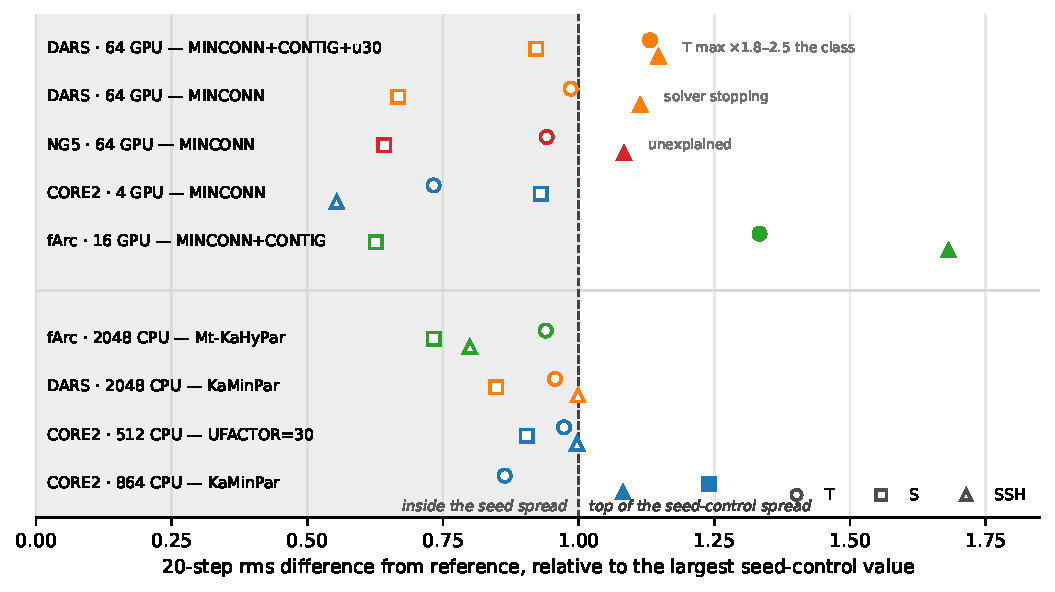
\includegraphics[width=0.92\textwidth]{fig_m11_disturbance.pdf}
\caption{\small Twenty-step rms difference from the reference for each candidate, by field,
divided by the largest difference the seed partitions of that same point produce (dashed line;
shaded region below it). Filled markers exceed the seed scatter. Every candidate shown
completed the 3{,}000-step run. At DARS 2{,}048 processes the scale uses the four seed
partitions that ran, the fifth being the step-14 divergence of Section~5; the
Hilbert-renumbered CORE2 candidate is compared under its own numbering and is not shown.}
\label{fig:dist}
\end{figure}

\emph{Within the seed scatter.} Most recommended candidates. At CORE2 on 4 GPU processes the
fastest candidate lies below every seed partition in all three fields; KaMinPar at DARS 2{,}048 lies
below every seed partition in temperature and salinity; Mt-KaHyPar at fArc and both CORE2 512
settings lie inside. These candidates are not distinguishable from the partition change a user
makes by rebuilding with a new seed.

\emph{Sea-surface height only, with a known cause.} The fastest DARS 64-GPU candidate ($-14.3\,\%$)
exceeds the seed scatter in sea-surface height alone, by 11\,\%. The barotropic solver stops
when the residual has fallen by a fixed factor, so a partition on which it converges faster
performs fewer iterations and stops at a different point inside the same tolerance. That is
what happens here: at DARS all three candidates need fewer iterations than any of the seed
partitions, and at CORE2 the candidate with the fewest iterations has the largest sea-surface
height difference. Both runs meet the tolerance the solver was asked for, and a tighter
tolerance would reduce the difference.

\emph{Sea-surface height only, cause unknown.} The fastest NG5 64-GPU candidate ($-9.8\,\%$) exceeds the
scatter by 8\,\% in sea-surface height, but its iteration counts match the seed partitions
step for step, so the mechanism above does not apply. We have no explanation for it.

\emph{Temperature or salinity.} Three candidates differ from the reference by more than the
seed partitions do in temperature or salinity: the $-19.7\,\%$ DARS candidate (temperature rms
$+13\,\%$, and a temperature maximum of 16.2 against 6.4--8.8 for the seed partitions), the
fArc GPU candidates (temperature rms $+18$ to $+33\,\%$), and KaMinPar at CORE2 864 (salinity
rms $+24\,\%$, temperature below every seed partition). Temperature and salinity carry the
model's long-term state, and an isolated maximum well outside the seed range is the same
pattern as the local runaways of Section~5 at an earlier stage. Before using one of these in
production, run it against the shipped partition for long enough to compare climatologies.

All numbers here come from twenty steps of a cold start. They show whether a partition change
is detectable against the change a new seed already makes; they say nothing about a
multi-decade integration. The cheap next test is to compare the model state after the
3{,}000-step run against the same seed partitions; the conclusive one is a multi-year pair of
integrations.

\section{Recommendations}

For FESOM2 upstream, in order of value:
\begin{enumerate}\itemsep2pt
\item Call \texttt{METIS\_PartGraphKway} in \texttt{fort\_part.c}, so that \minconn, \contig\
and the communication-volume objective reach METIS, and make the partitioner options run-time
switches instead of compile-time constants.
\item Adopt the 3{,}000-step test together with the options: every new partition, whatever
produced it, runs 3{,}000 steps at its target process count and the mesh's cold-start time
step before production use; a failure is answered by rebuilding with a new seed.
\item Rebuild the isolated-node repair in \texttt{check\_partitioning}, which currently takes
a single neighbour as reassignment candidate, and update METIS to 5.2.1.
\end{enumerate}

For runs on the machines measured here: use \minconn\ on GPU, and decide \contig\ and
\texttt{UFACTOR} by a timing run, since they help on some meshes and cost on others. On CPU
use KaMinPar or Mt-KaHyPar with $w = 100 + \mathrm{nlev}$, or \texttt{UFACTOR=30} if adding a
partitioning program to the workflow is not worth it (at CORE2 512 the two are equal; at DARS
2{,}048 the program is 1.1 percentage points better and the only candidate that both ran
3{,}000 steps and stayed inside the seed scatter). Hilbert renumbering is worth taking on
CORE2-class meshes where re-establishing the reference solutions is acceptable. Quantities
computed from a partition are useful for designing candidates and useless for accepting them:
acceptance is the 3{,}000-step run plus the comparison of Section~6.

\section{Status}

All measurements are complete. Four partitions --- the CORE2 GPU and CPU winners, fArc 2{,}048
and DARS 2{,}048 --- are packaged as mesh directories that carry their own run records; the
DARS and NG5 64-GPU partitions can be packaged the same way. What remains is the upstream pull
request.

Two questions are open. Whether an interconnect with working GPU-direct communication prices
messages like the A100 fabric or like the GH200 test system decides how much of the GPU gain
transfers to JUPITER, and only a measurement there will settle it. And for the three
candidates whose temperature or salinity difference exceeds the seed scatter --- among them the
largest gain measured, $-19.7\,\%$ on DARS --- a long paired integration would show whether the
difference matters at climate scale.

\vspace{4pt}
\noindent\textit{Job ids for every number quoted here, and the full record of the experiments,
are in \path{docs/PARTITIONING_M11.md}; the operational summary is
\path{docs/M11_RECOMMENDATION.md} and the complete table of timing runs is produced by
\path{scripts/m11_harvest_races.py} \texttt{--best}.}

\end{document}
